\chapter[Implementação do Serviço]{Implementação Do Serviço}

\section{Visão Geral}

Como proposto inicialmente, este trabalho de conclusão de curso visa a implementação de um Serviço que seja capaz de receber uma base de dados e aplicar os modelos de seleção de características, informando então quais são as características mais relevantes ao problema. Para alcançar tal feito, a biblioteca Weka \cite{weka_2005} foi selecionada. A biblioteca possui um acervo de métodos e algoritmos para mineração de dados muito bem implementados feitos em Java e C. A biblioteca é mantida pelo \textit{Machine Learning Group} da Universidade de Waikato e é código aberto, além de conter vários cursos de como utilizar a ferramenta.

A escolha dessa biblioteca foi feita pelo fato dela ser código aberto, e por ser bem completa, o que facilita implementar apenas os modelos de seleção de características, não tendo que focar na implementação dos classificadores.

O sistema foi desenvolvido em Ruby on Rails \cite{ror}, utilizando a linguagem JRuby \cite{jruby}. A escolha dessas ferramentas foi feita através da necessidade de um desenvolvimento rápido, e que pudesse haver uma comunicação com a linguagem Java, devido ao uso da biblioteca Weka. Ruby on Rails é conhecida pela agilidade na criação de aplicações Web, o que encaixava na necessidade de um desenvolvimento rápido, enquanto JRuby, por ser uma linguagem que utiliza-se de uma Java Virtual Machine, assim como o Java, consegue acessar bibliotecas Java e utiliza-las, sendo perfeita para uma integração com a biblioteca Weka.

\section{Arquitetura do Serviço}
A arquitetura do serviço foi pensada para que o usuário submetesse um arquivo contendo a base de dados em que ele gostaria que fosse realizado a Seleção de Características, sendo que esse arquivo deveria ser do formato \textit{.cvs} ou \textit{.arff}. Ao submeter esse arquivo ele passaria pelas análises necessárias no sistema que serão descritas na fase de Pré Processamento. Em seguida o usuário poderia executar essa base de dados utilizando um dos modelos descritos e demonstrados anteriormente, tal procedimento será melhor explicado na fase de Execução da Base de Dados, e por último, após o serviço executar a base ele deverá atualizar as informações de execução da base, informando quais foram as características selecionadas e qual a acurácia da em relação ao classificador kNN.

O Serviço utiliza-se da arquitetura mostrada na Figura 12.

\begin{figure}[h]
	\centering
	\label{fig13}
		\includegraphics[keepaspectratio=true,scale=0.35]{figuras/fig13.eps}
	\caption{Arquitetura do Serviço de Seleção de Características}
\end{figure}

Podemos ver que o sistema age em sua grande maioria no lado servidor, onde ele realiza o Pré Processamento, a Execução da base de dados, a Atualização do Status da Execução, e a Atualização os dados. Podemos perceber também o uso de Threads de processamento para que seja possível melhorar o desempenho do sistema, uma vez que o JRuby utiliza de Threads reais em seu processamento \cite{jruby}, fazendo com que o uso de Threads possua um resultado satisfatório.

Tendo essa visão da arquitetura do sistema, foi pensado como seria o relacionamento entre as diversas entidades do serviço, sendo as principais detalhadas na Figura 13

\begin{figure}[H]
	\centering
	\label{fig14}
		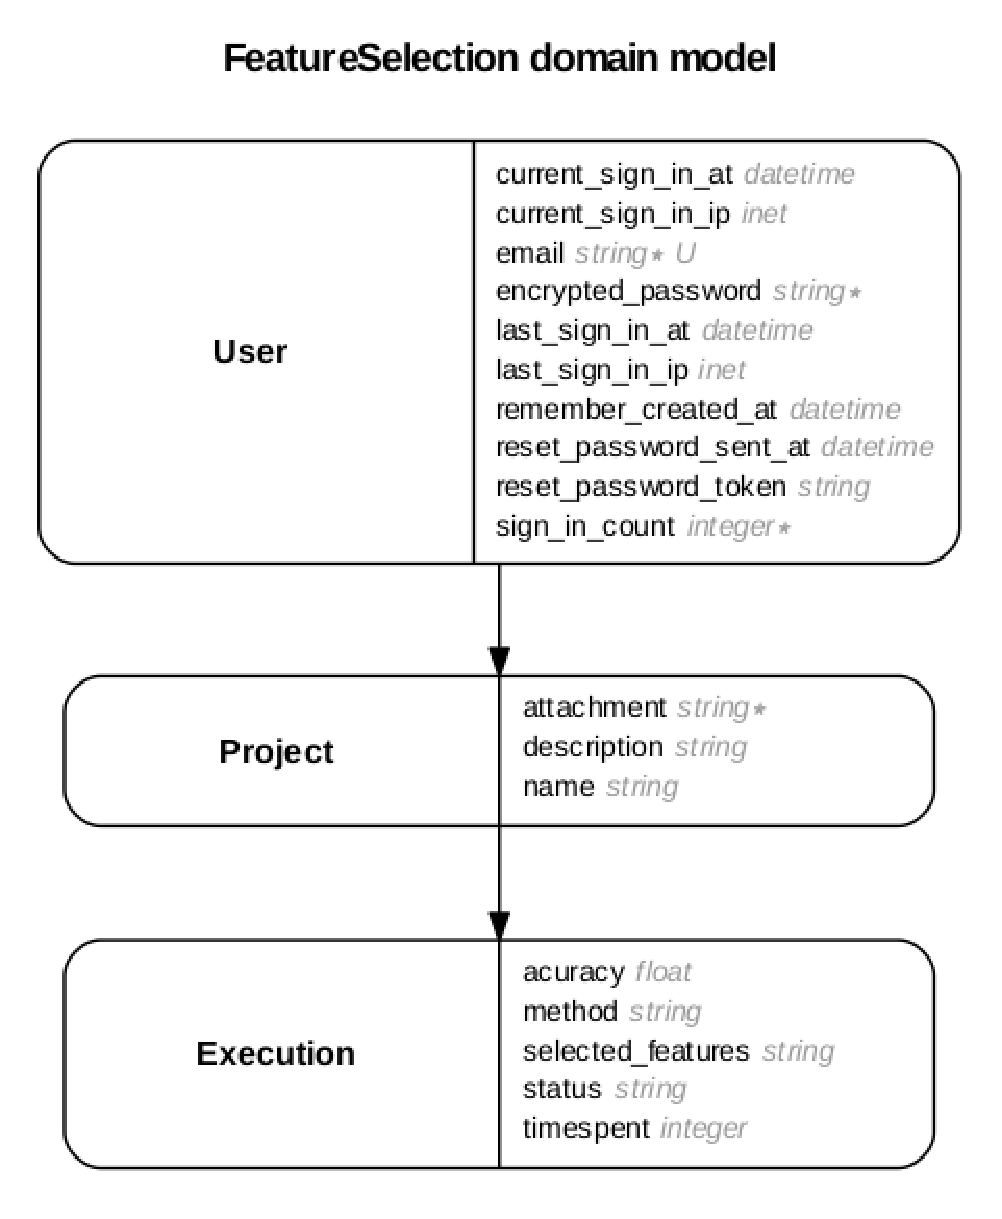
\includegraphics[keepaspectratio=true,scale=0.35]{figuras/fig14.eps}
	\caption{Diagrama de Classes do Serviço}
\end{figure}

\section{Fases do Serviço}
O serviço implementado segue as fases que estão listadas abaixo. Essas fases corroboram para o funcionamento da aplicação de modo que o seu fluxo de execução, mostrado ao final dessa seção, seja executado e, a partir disso, selecionar as características que sejam mais preponderantes ao problema de acordo com os métodos de seleção de características, conforme mostrado nos capítulos anteriores.
\subsection{Pré Processamento}

A fase de Pré Processamento é de suma importancia ao serviço pois a base de dados é adquirida nessa fase, e ao ser adquirida ela deve ser analisada para que seja possivel constatar a necessidade de algum tipo de pre processamento, tal como a conversão, pois a biblioteca Weka, que é utilizada para trabalhar as bases de dados, funciona apenas com arquivos do formato \textit{Attribute-Relation File Format} (.arff), sendo assim, qualquer base que não esteja nesse formato não será aceita, salvo a exceção do formato \textit{Comma-separated values} (.csv), onde é utilizado um conversor para que seja possível utilizar essa base se ele estiver no formato descrito na Figura 14.

\begin{figure}[H]
	\centering
	\label{fig15}
		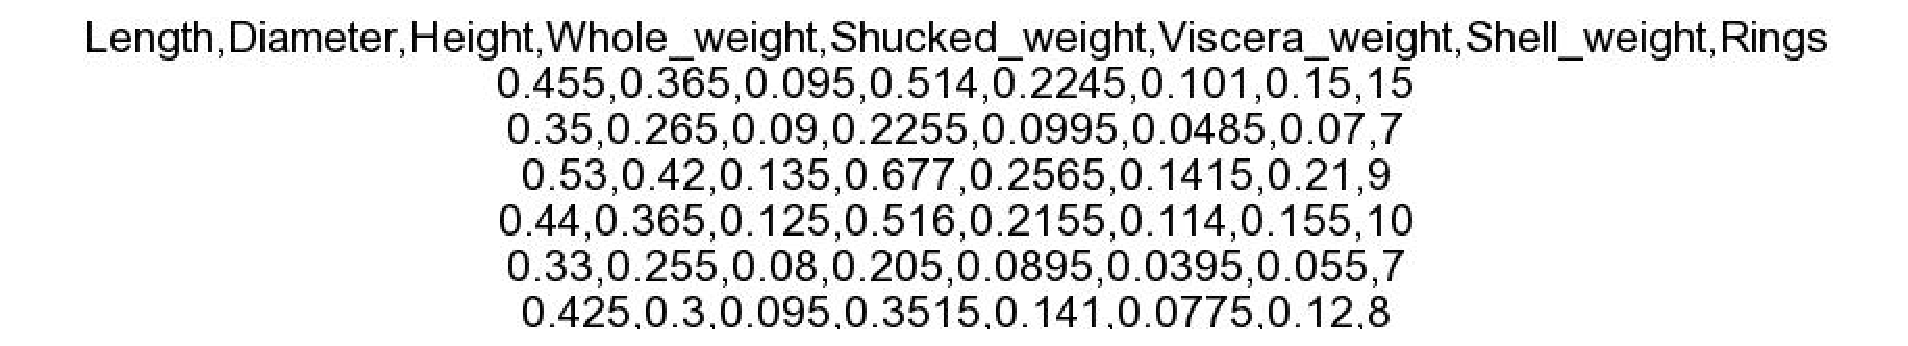
\includegraphics[keepaspectratio=true,scale=0.5]{figuras/fig15.eps}
	\caption{Arquivo Formato .csv}
\end{figure}

Conforme mostrado na figura, a primeira linha deve descrever o nome das características do problema, e as demais linhas devem compor os dados da base, estando cada um dos dados alinhados a sua característica. Percebe-se que todas as informações são separadas por vírgulas, e esse padrão deve ser mantido para que o conversor reconheça a estrutura do arquivo e consiga convertê-lo.

O resultado dessa conversão pode ser observado na Figura 15, onde é possível ver um arquivo .arff já convertido, e como ele é configurado.

\begin{figure}[H]
	\centering
	\label{fig15}
		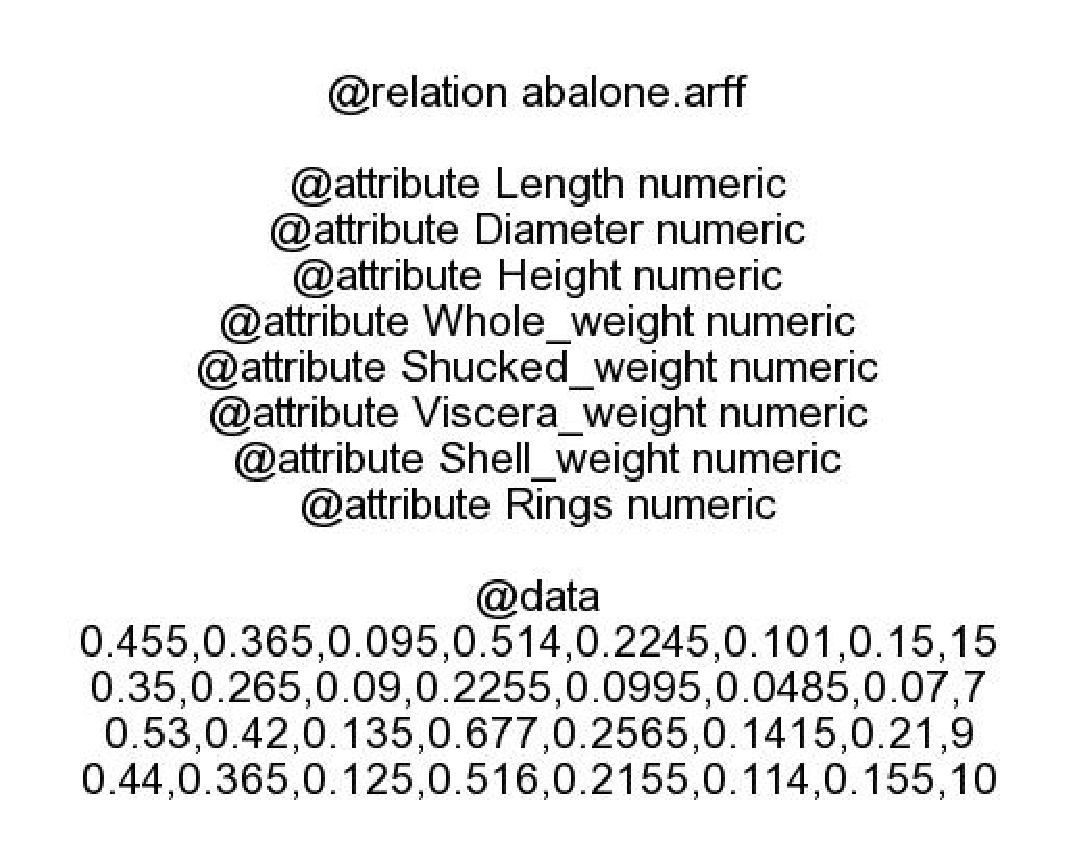
\includegraphics[keepaspectratio=true,scale=0.5]{figuras/fig16.eps}
	\caption{Arquivo Formato .arff}
\end{figure}

Podemos observar que na primeira linha existe o nome da base, depois é descrito cada uma das características e o seu tipo (numérico, nominal, etc. como já dito em capítulos anteriores). Após descrever cada uma das características, é descrito os dados que compõem essa base, seguindo o mesmo padrão que é seguido no .csv, ou seja, separados por virgula.

Além dessa analise da base, também é analisado se existem lacunas na base de dados. Essas lacunas são dados que não estão inclusos, ou seja, estão nulos, e esse tipo de lacuna tende a não ser aceito por alguns classificadores, além de gerar ruído ou atrapalhar o treinamento do modelo \cite{labic_2002}. Para mitigar esse problema o sistema substituirá todas as lacunas pela média, em caso de atributo quantitativo, ou pela moda, em caso de atributo qualitativo. O sistema assume essa abordagem para que se tente evitar o \textit{overfitting}, que é quando um modelo se ajusta aos dados de treinamento e não necessariamente consegue generalizar quando se recebe outros dados \cite{hawkins_2002}.

Após realizadas todas essas etapas, a base finalmente estará pronta para ser executada na fase de Execução da Base de Dados.


\subsection{Execução da Base de Dados}
Durante essa etapa, a base submetida na fase de Pré Processamento será submetida a um dos modelos selecionado pelo usuário, e que foram implementados e mostrados anteriomente neste trabalho, sendo eles: \textit{Relief-F, Decision Tree Method e Linear Forward Selection with kNN}. Cada um desses métodos será executado dentro de uma \textit{Thread} para que seja possível utilizar de todo o potencial da linguagem JRuby, pois ela tem suporte para \textit{Threads} reais \cite{jruby}, o que torna o uso de \textit{Threads} um bom artificio no sistema, deixando-o mais rápido para processar as bases.
\subsection{Atualização do Status da Execução}
Descrever como é feita a atualização do status da execução
\subsection{Atualização dos Dados}
Detalhar como os dados são atualizados e quais são eles
\subsection{Fluxo da Execução do Serviço}
Colocar uma imagem ilustrando o fluxo da execução do serviço
